Sequence to sequence learning (\ssl{}) aims to directly model the conditional
probability $p(\tgt{}|\src{})$ of mapping an input sequence,
$\src{1},\ldots,\src{n}$, into an output sequence, $\tgt{1},\ldots,\tgt{m}$.
It accomplishes such goal through the {\it encoder-decoder} framework proposed
by \citet{sutskever14} and \citet{cho14}. As illustrated in Figure~\ref{f:s2s},
the {\it encoder} computes a representation $\MB{s}$
for each input sequence. Based on that input representation,
the {\it decoder} generates an output sequence, one unit at a time, and hence, decomposes the conditional probability as:
\begin{equation}
\log p(\tgt{}|\src{}) = \sum_{j=1}^m \nolimits \log
p\open{\tgt{j}|\tgt{<j},\src{},\MB{s}}
\label{e:s2s}
\end{equation}


\begin{figure}%[tbh]
\centering
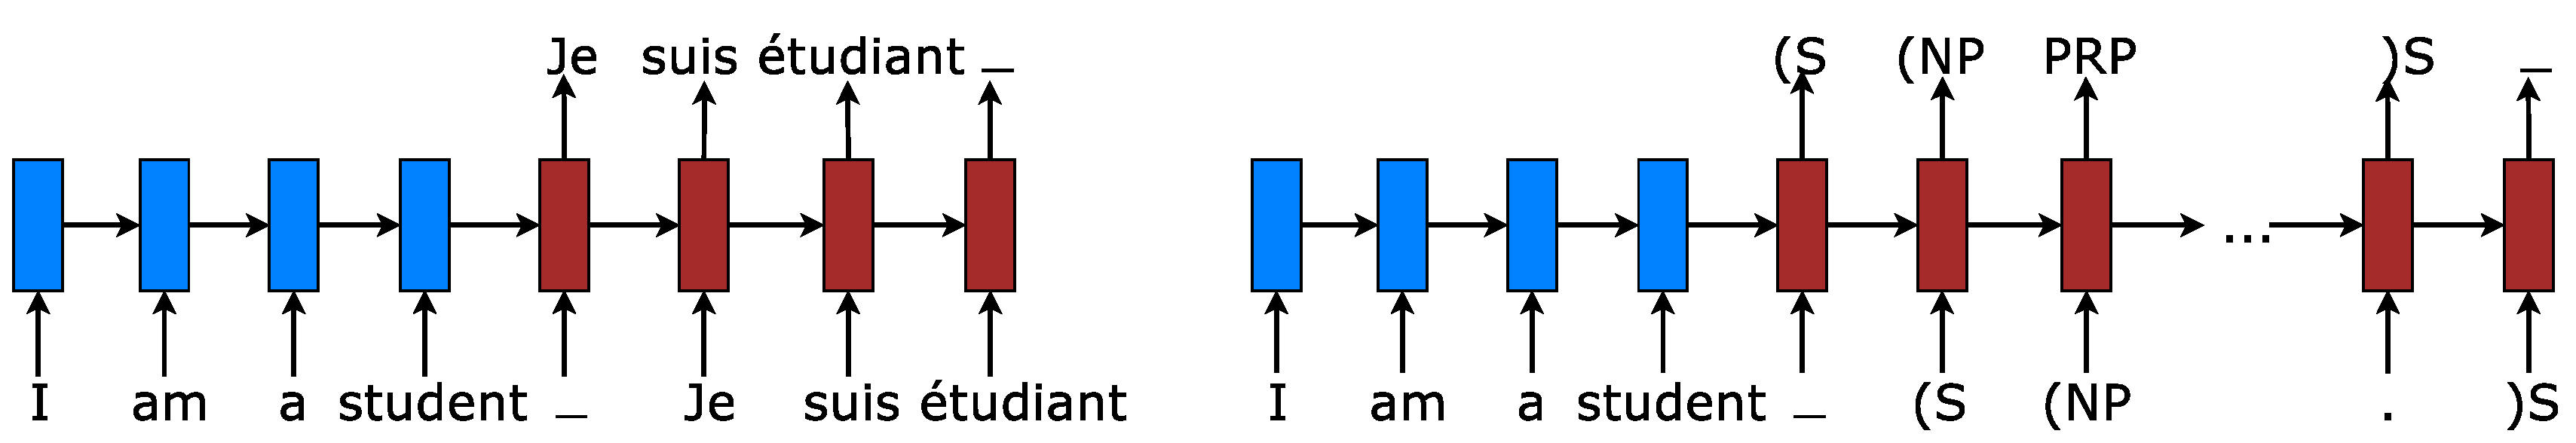
\includegraphics[width=1\textwidth, clip=true, trim= 0 0 0
0]{img/6-1_seq2seq}
\caption[Sequence to sequence learning examples]{{\bf Sequence to sequence learning examples} -- (left) machine
translation \citep{sutskever14} and ({\it right}) constituent parsing
\citep{vinyals15grammar}.}
\label{f:s2s}
\end{figure}

A natural model for sequential data is the recurrent
neural network (RNN), which is used by most of the recent \ssl{} work.
These work,
however, differ in terms of: (a) {\it architecture} -- from unidirectional, to
bidirectional, and deep multi-layer RNNs; and (b) {\it RNN type} -- which are long-short term memory (LSTM)
\citep{lstm97} and the gated recurrent unit \citep{cho14}. 

Another important difference between \ssl{} work lies in what constitutes the
input representation $\MB{s}$.
The early \ssl{} work \citep{sutskever14,cho14,luong15,vinyals15caption} uses only the last encoder state
 to initialize the decoder and sets $\MB{s}\!=\![\text{ }]$ in %\textrm{RNN encoder}(x) for each $j$ 
\eq{e:s2s}. Recently, \citet{bog15} proposes an {\it attention mechanism}, a way
to provide \ssl{} models with a random access memory, to 
handle long input sequences.
This is accomplished by setting
$\MB{s}$ in \eq{e:s2s} to be the set of encoder hidden states already computed. On the decoder side, at each time step, the attention mechanism will
decide how much information to retrieve from that memory by learning where to
focus, i.e., computing the alignment weights for all input positions. Recent work such as \citep{xu15,jean15,luong15attn,vinyals15grammar}
has found that it is crucial to empower \ssl{} models with the attention mechanism.

